\subsection{By spectral shift}
\label{sec:rth:lambda}

We can write the thermal resistance from (\ref{eq:rth})
as \cite{Heinen2012,Giet2008}
\begin{equation}
\Rth = \pd{T}{D} = \pd{\lambda}{D}/\pd{\lambda}{T}.
\label{eq:rth_long}
\end{equation}
In this description
$\lambda$ corresponds to
the longest emitted wavelength.
The longest emitted wavelength is said to
correspond to the hottest part of the VECSEL.
This is a result of the predominantly linear shift
in refractive index
as function of temperature \cite{Heinen2012}.
This approach ignores
the change in cavity length
resulting from thermal expansion.

The longest emitted wavelength
is correlated
with dissipated power.
This gives a linear relation
for each heat sink temperature
\begin{equation}
\lambda_{\Ths} = \left.\pd{\lambda}{D}\right|_{\Ths} D + \lambda_{0,\Ths}.
\end{equation}
By substituting
\begin{equation}
\lambda_{0,\Ths} = \pd{\lambda}{T} \Ths + \lambda_0
\end{equation}
we end up with \cite{Heinen2012}
\begin{equation}
\lambda = \pd{\lambda}{D} D + \pd{\lambda}{T} \Ths + \lambda_0,
\label{eq:rth_fit}
\end{equation}
from where we can extract
the required parameters for (\ref{eq:rth_long})
using linear regression.

We record the emitted spectrum
for every pump setting.
In order to determine
the longest emitted wavelength
we cut
these spectra
as indicated
in Fig.~\ref{img:longest_wavelength}.
By measuring each pump setting multiple times,
we can increase our confidence
in the extracted wavelength value.

\begin{figure}
\centering
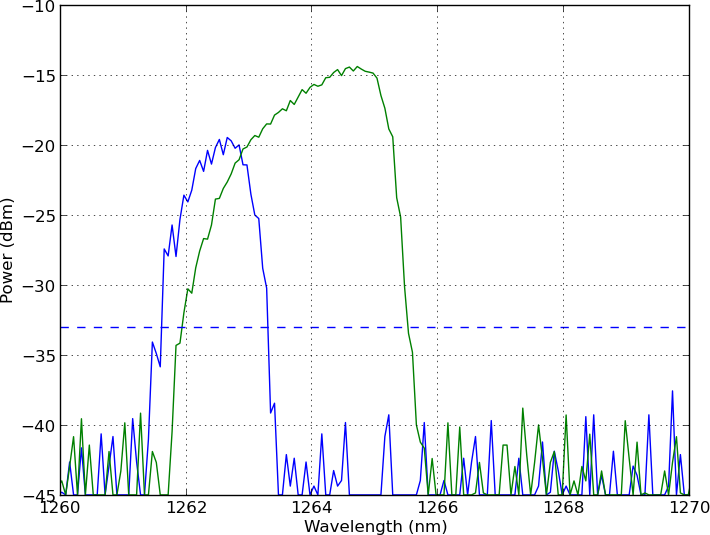
\includegraphics[width=10cm]{img/longest_wavelength.png}
\caption{We cut the spectrum
at a level
above the noise floor.
For each pump setting
we have multiple measurements,
giving us a margin
of how reliable this extracted
longest wavelength is.}
\label{img:longest_wavelength}
\end{figure}

The dissipated power $D$
corresponds to the left-over power
of the pump ($P$),
after we have accounted for the
reflected ($R$) and emitted ($E$) part
\cite{Heinen2012},
\begin{equation}
D = P - R - E.
\label{eq:dissip}
\end{equation}